\part{Data types}
\frame{\partpage}

\begin{frame}{What is a type?}
	\begin{itemize}
		\pause\item A \textbf{variable} in Python holds a \textbf{value}
		\pause\item Every value has a \textbf{type}
		\pause\item The type of a value dictates:
			\begin{itemize}
				\pause\item What sort of data it can hold
				\pause\item How the data is stored in memory
				\pause\item What operations can be done on it
			\end{itemize}
	\end{itemize}
\end{frame}

\begin{frame}{Memory}
	\pause
	\begin{center}
		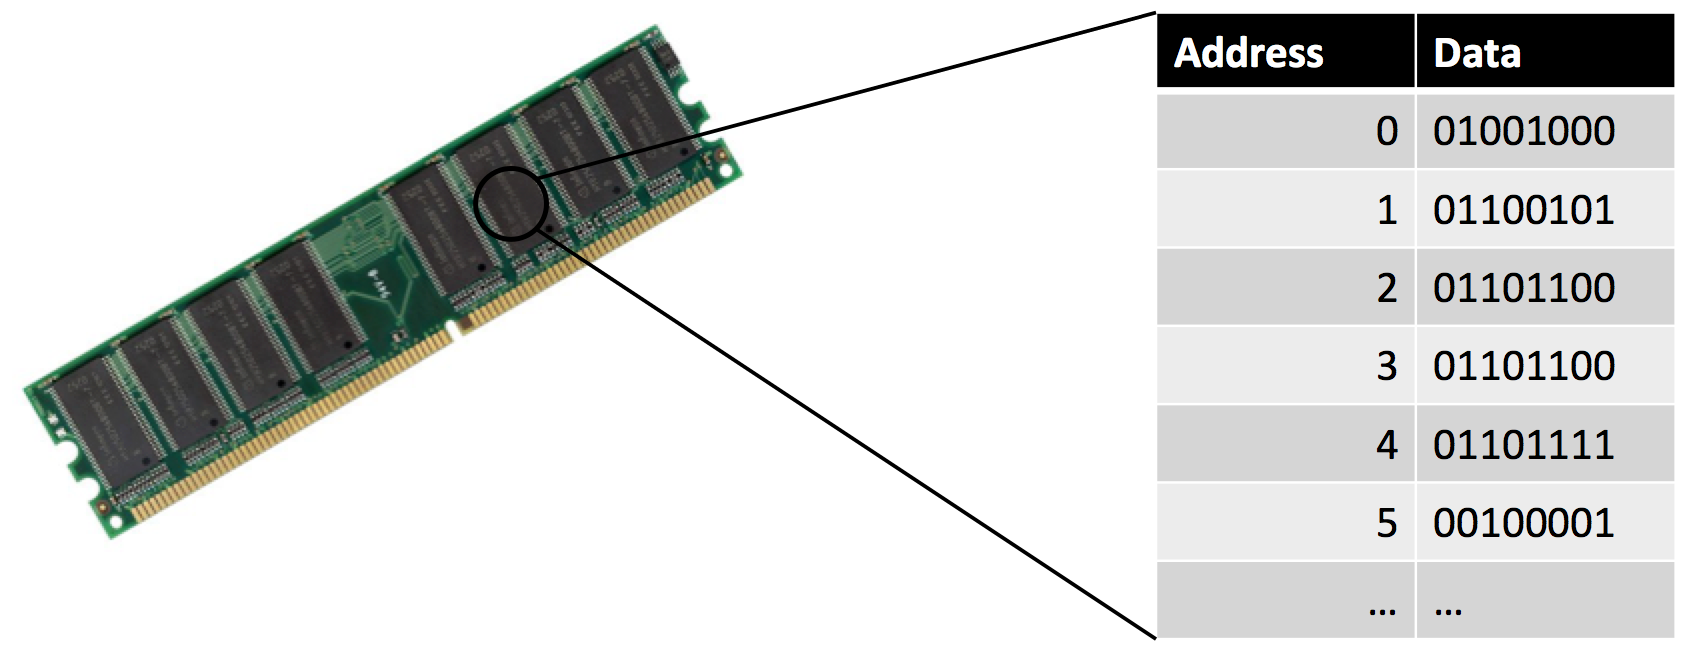
\includegraphics[width=0.8\textwidth]{memory}
	\end{center}
	\begin{itemize}
		\item Memory works like a set of \textbf{boxes}
		\pause\item Each box has a number, its \textbf{address}
		\pause\item Each box contains a \textbf{byte} (8 bits)
	\end{itemize}
\end{frame}

\begin{frame}{Data representation} 
	\begin{itemize}
		\pause\item All data is stored as \textbf{sequences of bytes}
			\begin{itemize}
				\pause\item Sequence of bits, in multiples of 8
				\pause\item Sequence of numbers between 0--255
			\end{itemize}
	\end{itemize}
\end{frame}

